\begin{figure}[t!]
  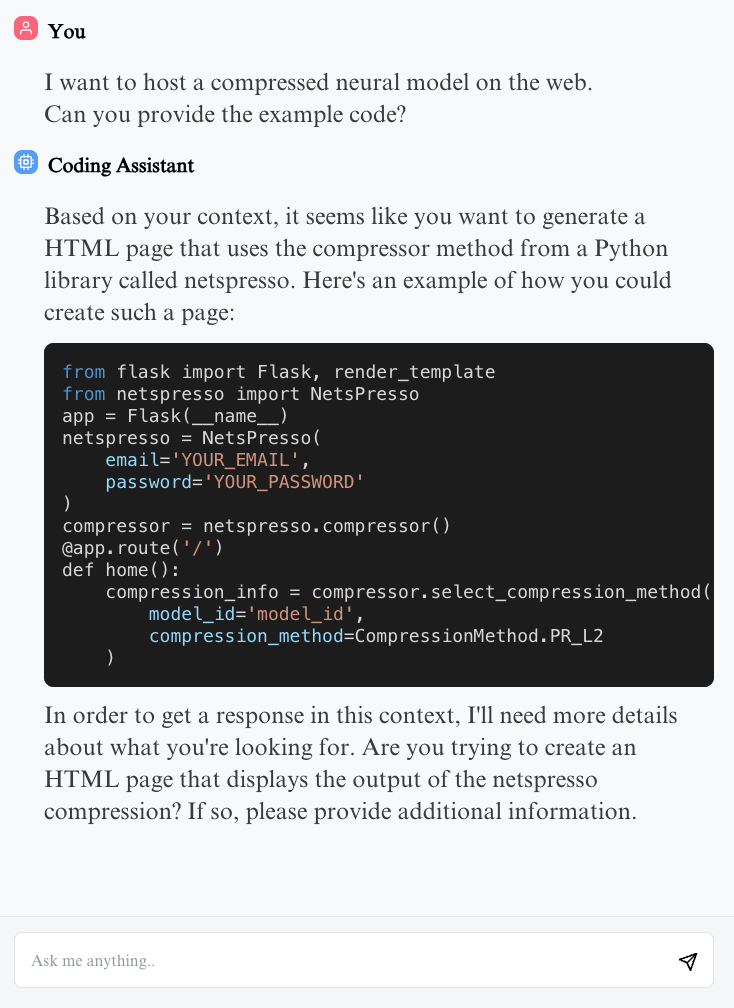
\includegraphics[width=\columnwidth]{figures/fig_1.png}
  \caption{An example of an LLM generating plausible code even when the request is made outside the functionality provided by the library. When generating code based on the API documentation of NetsPresso~\cite{netspresso2024}, a deep learning model optimization library, an LLM generates the response to a query requesting web page creation using Netspresso API.}
  \label{fig:1}
\end{figure}
\section{Introduction}
Recently, the large language models (LLMs) have demonstrated unprecedented performance on a variety of natural language processing tasks. Based on their language understanding and generation capabilities, they are now widely used as coding assistants to support developers across various industries. This has significantly improved software development productivity. In particular, Retrieval-augmented Generation (RAG)~\cite{shuster2021RAGreducehalu} has enabled LLMs to generate code for various libraries that they were not trained on.
As depicted in Figure~\ref{fig:1}, when generating code through Retrieval-augmented Code Generation (RaCG), LLMs often produce plausible but incorrect code for a user's query, which may not be answerable. Developers using these code assistants in a RaCG environment may often ask questions that fall outside the capabilities provided by the library because they are not proficient in using it. Therefore, in such cases, LLMs must be able to determine whether they can provide an answer before generating a response code for the user's query.

\begin{figure*}[t!]
    \centering
    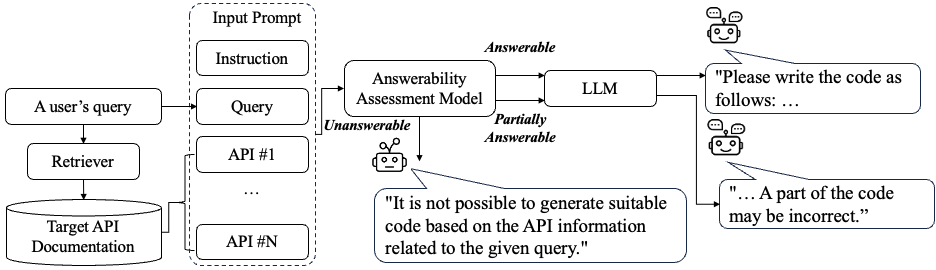
\includegraphics[width=1.0\linewidth]{figures/fig_2.png}
    \caption{The process of evaluating the answerability of a user's query in RaCG and generating code accordingly or rejecting code generation}
    \label{fig:2}
\end{figure*}


This can be seen as a well-known hallucination problem. Although RAG is known to mitigate the hallucination by making the language model's response grounded on external knowledgebase, the hallucination still exists~\cite{esetal2024ragas,li-etal-2024-llatrieval}. To reduce such hallucinations, various methods for detecting hallucinations have been studied. SelfCheckGPT~\cite{manakul2023selfcheckgpt} uses the consistency of multiple sampled responses to determine whether generated responses include hallucination. This method requires the sampling of a large number of responses to determine hallucination. RAGAS~\cite{esetal2024ragas} and LLatriEval ~\cite{li-etal-2024-llatrieval} examine whether the responses generated in a RAG scenario are well-supported by the documents. However, these methods all require the generation of responses by the LLM one or multiple times. 
As an alternative to approach hallucination, one can think of assessing the answerability of the input prompt before LLM generates the response. There has not been much research on this task in the RaCG scenario. If it is possible to evaluate answerability without generating multiple responses, it could reduce computational costs for LLM service providers. Additionally, users would be able to reduce their waiting time for responses and modify their queries to receive the desired answers more quickly. This study discusses the task of evaluating such answerability.

Moreover, various benchmarks have been proposed to evaluate hallucinations in LLMs including general \cite{li2023halueval} and code domain~\cite{tian2024codehalu}. Most work addresses the issue of determining whether the generated responses are hallucination. However, to the best of our knowledge, there is no dataset available for assessing whether the given queries themselves are answerable. In this study, we build and release a benchmark dataset, \textbf{R}etrieval-\textbf{a}ugmented \textbf{C}ode \textbf{G}enerability \textbf{Eval}uation (RaCGEval), annotated for whether the queries given in RaCG are answerable.

Our contributions can be summarized as follows:
\begin{itemize}
  \item We propose methods to construct a benchmark for assessing the answerability of users' queries in RaCG. 
  \item We publicly release the RaCGEval benchmark. 
  \item We built models to evaluate the answerability of given users' queries and conducted an in-depth investigation on this task.  
\end{itemize}
RaCGEval benchmark dataset and pre-trained answerability assessment models are publicly available. \footnote{ \url{https://github.com/Nota-NetsPresso/RaCGEval}}